\chapter{\Idx{Electrokinetics}}
\noindent
\modinfo{Module name}{\Idx{Electrokinetics}}
\modinfo{Module subroutines}{helmholtz\_smoluchowski1, helmholtz\_smoluchowski2,\\ helmholtz\_smoluchowski3, helmholtz\_smoluchowski, getJouleHeat}
\modinfo{Module author}{Thomas Zwinger}
\modinfo{Document author}{Thomas Zwinger}
\modinfo{Document created}{April 13th 2005}

\section{Introduction}

If dealing with electrolytic fluids constrained to small volumes, surface forces caused by electric surface charges in combination with externally applied electrostatic fields are sufficient strong to affect the fluid volume. If these effects are utilized to attenuate the fluid volume, we talk of \textit{Electrokinetics}. The term \textit{Electroosmotic Flow} (EOF) is used in connection with the attenuation of a net charge inside a originally neutral electrolyte caused by separation induced by a surface charge of a wall.

In most applications utilizing EOF, externally applied fields are sufficient small in order to justify neglecting electric heating (Joule heating) inside the fluid volume. Nevertheless, certain applications, such as High Voltage Capillary Electrophoresis (HV-CE), demand the consideration of this effect \cite{KnoMcC1994}.

\section{Theory}
Chemical reactions between the contents of a liquid and the wall material may lead to a net charge of the containment at the wall-liquid interface. If the liquid is an electrolyte (i.e., it contains free ions), ions of opposite charge align along the wall creating the \textit{Stern layer}. Adjacent to the Stern layer, a charge separation - called the \textit{diffuse layer} of the initially neutral electrolyte takes place. Due to the two layer structure the whole are area of charge separation in the vicinity of a wall is called the \textit{Electric Double layer} (EDL). 
\begin{figure}[tbhp]
\vspace{-11cm}
\centerline{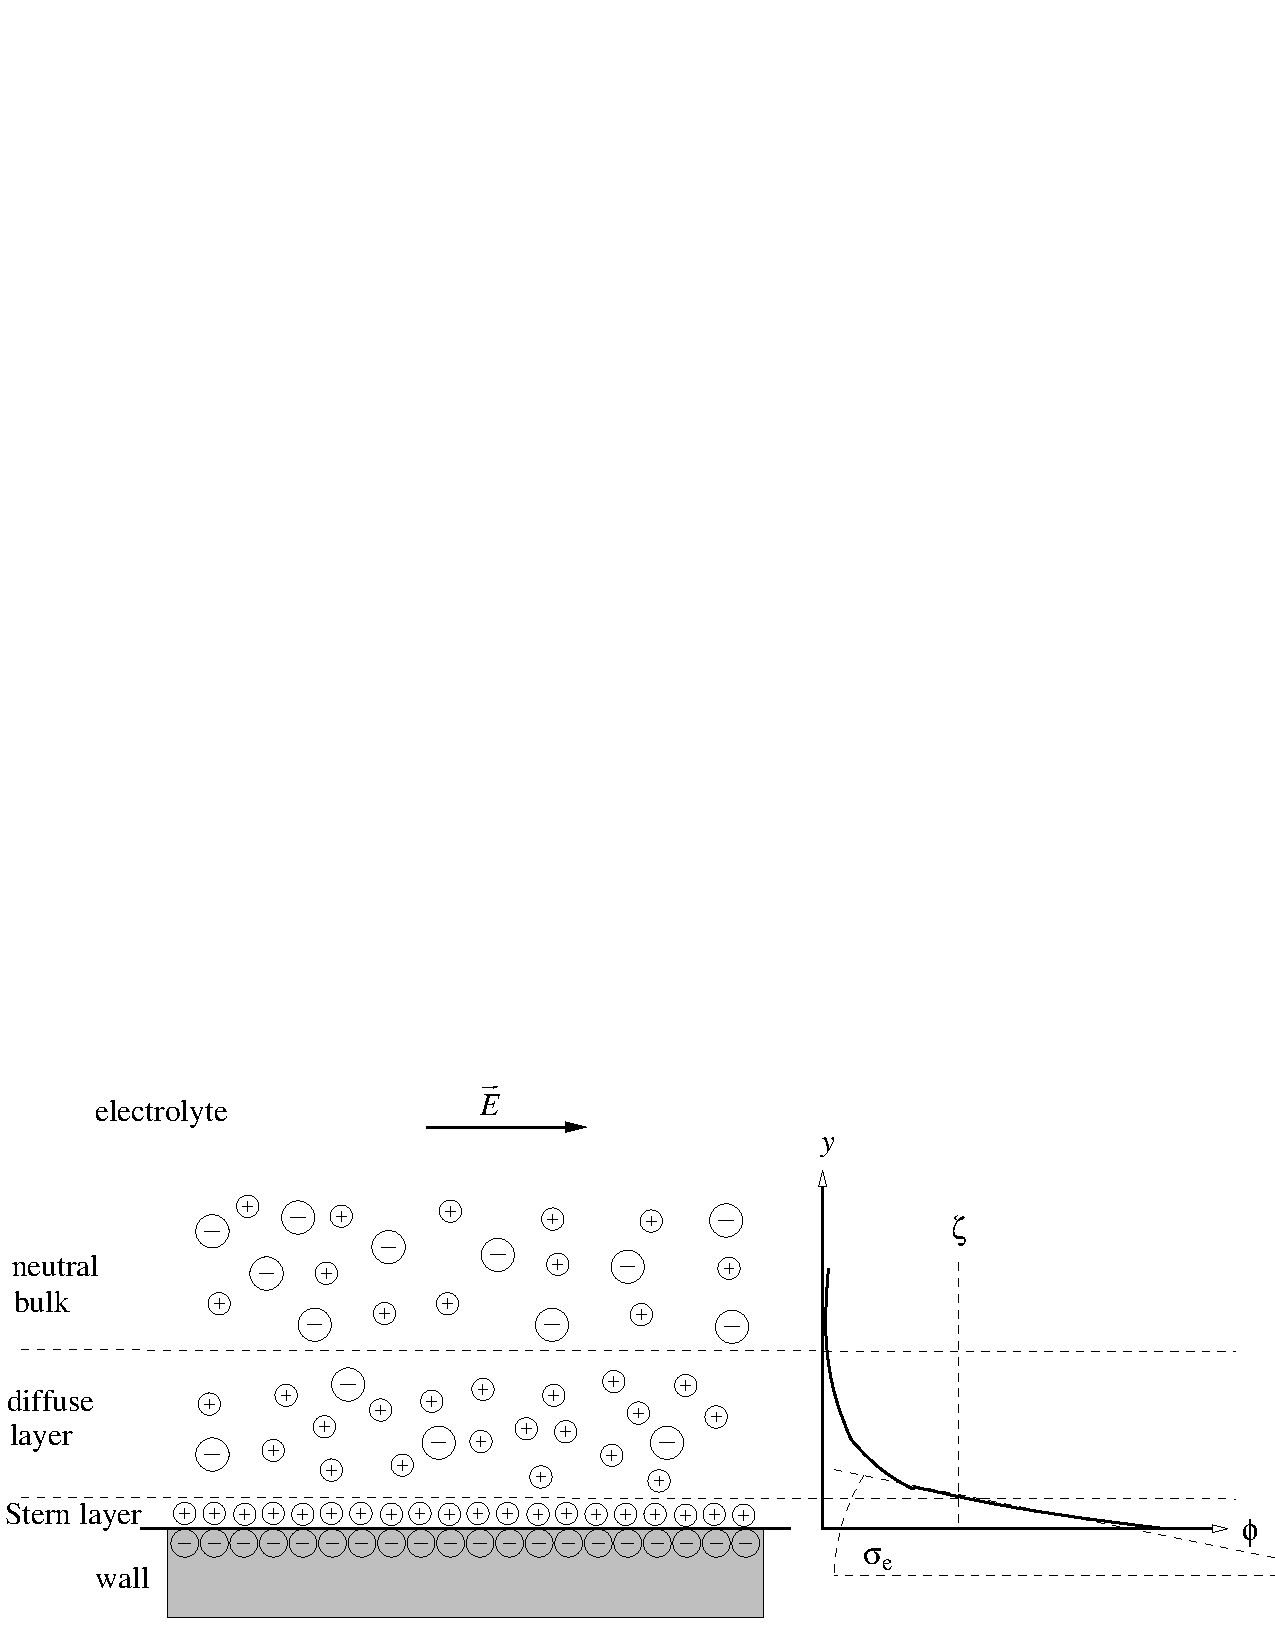
\includegraphics[width=0.9\textwidth]{EDL_bw.pdf}}
\caption{\label{ek:Fig.EDL} Structure of the EDL. The value of the induced potential, $\Phi$ at the Stern layer usually is referred to as the zeta-potential, $\zeta$}
\end{figure}
\subsection{Electroosmotic slip velocity}\label{EOF}
Considering a symmetric electrolyte -- i.e., the bulk ion density of ions with opposite valence numbers $\pm z$ are equal $n^{+}_{0}=n^{-}_{0}=n_{0}$ --  at a certain temperature, $T$, the typical width-scale of the EDL is given by the \textit{Debye length} \cite{KarBes:2001}
\begin{equation}\label{ek:debye}
\lambda_{\mathrm{D}} = \left(\dfrac{\epsilon_{\mathrm{f}}\epsilon_{0}\,k_{\mathrm{b}}\,T_{0}}{2\, n_{0}\, z^{2}\, e^{2}_{0} }\right)^{1/2}.
\end{equation}
Here $e_{0}$ stands for the unit charge and $k_{\mathrm{b}}$ denotes the Boltzmann constant. The relative permittivity of the electrolyte and the permittivity of vacuum are given by $\epsilon_{\mathrm{f}}$ and $\epsilon_{0}$, respectively. 


The potential, $\Phi$ and the volume charge density, $\rho_{e}$, within the EDL are tightly coupled to each other by the Poisson-Boltzmann equation \eqref{eq:poisson-boltzmann} (see chapter \ref{poisson-boltzmann}). In order to exactly resolve the dynamics close to the walls, \eqref{eq:poisson-boltzmann} should be solved and the resulting specific electric force then be considered in the equation of motion. Nevertheless,  provided the typical length scales of the flow perpendicular to the containment walls, $H$, strongly exceed those of the EDL -- in other words, we obtain very small values for the non-dimensional group $\mathcal{L} = \lambda_{\mathrm{D}}/H \ll 1$ -- the dynamics of the electrolyte inside the EDL does not have to be resolved at all. In this case simple considerations of a force balance between shear stress and electric force lead to a slip condition for the fluid \cite{YaFuLi:2001}. At the boundary, the tangential velocity is set to the \textit{Helmholtz-Smoluchowski} velocity
\begin{equation}
\label{ek:helm-smol}
\vec{u}_{\mathrm{tang.}}=\vec{u}_{\mathrm{H-S}} = \frac{\vec{E}_{\mathrm{tang.}}\epsilon_{\mathrm{f}}\epsilon_{0}\zeta}{\mu_{\mathrm{f}}},
\end{equation}
with $\mu_{\mathrm{f}}$ standing for the local fluid viscosity. The \textit{zeta potential}, $\zeta$ -- a property depending on the electric properties of the wall material as well as the electrolyte -- usually is determined experimentally. From a physical point of view it can be interpreted as the value of the solution obtained by \eqref{eq:poisson-boltzmann} at the Stern layer. The tangential component, $\vec{E}_{\mathrm{tang.}}$,  of the external electric field, $\vec{E}$, is evaluated from the outward pointing surface normal $\vec{n}$, applying the following relation
\begin{equation}
\label{ek:etang}
\vec{E}_{\mathrm{tang.}} = \vec{E} - \left(\vec{E}\cdot\vec{n}\right)\vec{n}
\end{equation}
Alternatively, the resulting slip velocity may be related to the tangential field using the \textit{Electroosmotic Mobility}, $\mu_{\mathrm{EOF}}$
\begin{equation}
\label{ek:HS-EOF-mobility}
\vec{u}_{\mathrm{H-S}} = \mu_{\mathrm{EO}}\,\vec{E}_{\mathrm{tang.}}.
\end{equation}
A combination of \eqref{ek:helm-smol} and \eqref{ek:HS-EOF-mobility} leads to the following identity
\begin{equation}
\label{ek:EOF-mobility}
\mu_{\mathrm{EO}} =\frac{\epsilon_{\mathrm{f}}\epsilon_{0}\zeta}{\mu_{\mathrm{f}}}.
\end{equation}

\subsection{Joule Heating}
Due to the small volume in microfluidic applications the additional heat produced by the external electric field needs to be considered. With the local electric conductivity, $\sigma$, and the local volume density, $\rho$, of the electrolyte the specific heat contribution by Joule heating from an external electric field, $\vec{E}$, is given by
\begin{equation}
\label{ek:joule-heating}
h = \sigma\,\vec{E}\cdot\vec{E}/\rho.
\end{equation}
The expression above can be added as body force to the heat transfer equation \eqref{heat_equation}.

\section{Limitations}
\begin{itemize}
\item The Helmholtz-Smoluchowski velocity should not be applied if the non-di\-men\-sion\-al group $\mathcal{L}$ defined in \ref{EOF} is of unity order or larger. Then the potential- and charge density distribution as well as the dynamics of the electrolyte inside the EDL has to be resolved. 
\item In a strict sense, the Helmholtz-Smoluchowski theory applies only to configurations where the normal-component of the external field, $\vec{E}\cdot\vec{n}$, is small. If dealing with electric insulating wall materials -- as it is usually the case in microfluidic applications -- this condition is implicitly complied with. 
\item The assumption of a Newtonian fluid underlies the derivation of the Helmholtz-Smoluchowski velocity.
\item The function \texttt{helmholtz\_smoluchowski} can only be applied on  boundaries of two-dimensional domains, where the tangential direction is uniquely defined.
\item The functions \texttt{helmholtz\_smoluchowski\{1,2,3\}} cannot be applied with a number larger than the dimension of the domain.
\end{itemize}


\section{Keywords}

\subsection{Keywords for helmholtz\_smoluchowski}

\sifbegin

  \sifitemnt{Constants}{}
  \sifbegin
  \sifitem{Permittivity Of Vacuum}{Real [8.8542e-12 C$^2$/Nm$^2$]}
   permittivity of vacuum, only needed if Helmholtz-Smoluchowski velocity is defined using expression \eqref{ek:helm-smol}
  \sifend

  \sifitemnt{Equation}{equation id}
  \sifbegin
    \sifitem{Electric Field }{String  [\texttt{computed}, \texttt{\tt constant}]} 
    the option for how to evaluate the electric field should be set to one of these values.\newline
    If set to  \texttt{computed}, the function will search for \texttt{Electric Field \{1,2,3\}} in the list of solver variables. If set to \texttt{constant}, the function will search for \texttt{Electric Field \{1,2,3\}} in the section \texttt{Material material id}, where \texttt{material id} is the id-number associated with the material parameter list of the electrolyte
  \sifend

  \sifitemnt{Material}{material id} \newline
  If the Helmholtz-Smoluchowski velocity is defined using expression \eqref{ek:helm-smol}, then the following keywords have to be provided in this section
  \sifbegin
   \sifitem{Viscosity}{Real}
   viscosity of the electrolyte
   \sifitem{Density}{Real}
  volumetric density of the electrolyte
   \sifitem{Relative Permittivity}{Real}
   relative permittivity of the electrolyte
  \sifend
%   Alternatively, the user can declare the EO-mobility, as explained in \eqref{ek:EOF-mobility}

  \sifitemnt{Boundary Condition}{bc id} \newline
  In two-dimensional configurations the Helmholtz-Smoluchowski velocity directly can be assigned to the tangential component of the velocity field
  \sifbegin
    \sifitemnt{Normal Tangential Velocity}{Logical True}
    \sifitem{Velocity 2}{= Variable Dummyargument\\ Real Procedure "Electrokinetics"\ "helmholtz\_smolu\-chowski"}
          Sets tangential EO slip velocity
  \sifend
  The argument \texttt{Dummyargument} can be any existing variable, since it is not used to evaluate the velocity.\newline
  In three-dimensional configurations (and as an alternative also in two-dimensional), the velocity has to be defined for each component
  \sifbegin
    \sifitemnt{Normal Tangential Velocity}{Logical False} 
    \sifitemnt{Velocity 1}{= Variable Dummyargument\\ Real Procedure "Electrokinetics"\ "helmholtz\_smolu\-chowski1"}
    \sifitemnt{Velocity 2}{= Variable Dummyargument\\ Real Procedure "Electrokinetics"\ "helmholtz\_smolu\-chowski2"}
    \sifitemnt{Velocity 3}{= Variable Dummyargument\\ Real Procedure "Electrokinetics"\ "helmholtz\_smolu\-chowski3"}
  \sifend
  The argument \texttt{Dummyargument} can be any existing variable, since it is not used to evaluate the velocity.\newline
  If the Helmholtz-Smoluchowski velocity is defined using expression \eqref{ek:helm-smol}, then the zeta potential, $\zeta$, for the specific boundary region has to be defined
  \sifbegin
    \sifitem{Zeta Potential}{Real}
    Sets the zeta-potential for this boundary
  \sifend
  Alternatively, the user can declare the EO-mobility, as explained in \eqref{ek:EOF-mobility}
    \sifbegin
    \sifitem{EO Mobility}{Real}
        Sets EO mobility for this boundary
  \sifend
\sifend
\subsection{Keywords for getJouleHeat}
\sifbegin
  \sifitemnt{Equation}{equation id}
  \sifbegin
    \sifitem{Electric Field }{String  [\texttt{computed}, \texttt{constant}]} 
    the option for how to evaluate the electric field should be set to one of these values.\newline
    If set to  \texttt{computed}, the function will search for \texttt{Electric Field \{1,2,3\}} in the list of solver variables. If set to \texttt{constant}, the function will search for \texttt{Electric Field \{1,2,3\}} in the section \texttt{Material material id}, where \texttt{material id} is the id-number associated with the material parameter list of the electrolyte
  \sifend

  \sifitemnt{Material}{material id}
   \sifbegin
    \sifitem{Electric Conductivity}{Real}
     electric conductivity of the electrolyte
    \sifitem{Density}{Real}
     volumetric density of the electrolyte
   \sifend

  \sifitemnt{Body Force}{bodyforce id}
   \sifbegin
    \sifitem{Heat Source}{= Variable Dummyargument \\ Real Procedure "Electrokinetics"\ "getJouleHeat"}
     adds specific heat source for \texttt{HeatSolve}.  
     The argument \texttt{Dummyargument} can be any existing variable, since it is not used to evaluate the Joule heating	
   \sifend
\sifend


\bibliography{elmerbib}
\bibliographystyle{plain}


